\documentclass[conference]{IEEEtran}
%\renewcommand{\thesubsection}{\thesection.\alph{subsection}}

%\addtolength{\oddsidemargin}{-.875in}
%\addtolength{\evensidemargin}{-.875in}
%\addtolength{\textwidth}{1.75in}
%\addtolength{\topmargin}{-.875in}
%\addtolength{\textheight}{1.75in}
	
\usepackage{bm}
\usepackage{amsmath}
\usepackage{amssymb}
\usepackage{tikz}
\usetikzlibrary{automata,positioning}
\usepackage{url}
\usepackage{float}
\usepackage{setspace}
\usepackage{filecontents,lipsum}
\usepackage[noadjust]{cite}
\usepackage{listings}


\begin{document}
%\raggedright
%\doublespacing

\title{A Survey on Machine Learning: Code Smells and Antipatterns}
\author{Rodger Byrd\\rbyrd2@uccs.edu}

\maketitle

\section{Abstract}
Recently, machine learning methods have been applied to detect and correct code smells, but this is a new field and it is not mature.

\section{Introduction}
A good overview of code smells is covered in \textit{A Survey on software smells} \cite{sharma_survey_2018}. 
The paper only mentions For my next detailed read I chose a paper called  \textit{A systematic literature review: Refactoring for disclosing code smells in object oriented software} \cite{singh_systematic_2018}. 

All cause confusion to the reader of the code. Developers spend more time reading than writing (citation?) code. If thesee smells and antipatterns can be detected and corrected, it will lead to more sustainable, more stable code with less time spent by the developer so less cost as well.

There are five types of code smell detection\cite{lafi_code_2019}, they are:
\begin{enumerate}
\item Metrics based smell detection
\item Rules/heuristic-based smell detection
\item History based smell detection
\item Optimization based smell detection
\item Machine Learning based smell detection
\end{enumerate}

\subsection{Code Smells and Antipatterns}
Code smells are similar to antipatterns, but code smells may not always be bad.
I've also seen antipatterns referred to as Atoms of Confusion \cite{gopstein_understanding_2017} and nano patterrns, which are very small anti-patterns like the size of a single method. 
An example of confusing code is shown below in in \ref{pattern1}.
Some developers will expect the output to be 25 and some will be 13 because they don't understand intuitively how the macro function works (the correct answer is 13).

\begin{lstlisting}[language=C,frame=single,caption=Example Atom of Confusion,label=pattern1]
#DEFINE M 2+3

int main() {
  int x=5, y;
  y= x * M;
  cout << y << endl;
  return 0;
}
\end{lstlisting}

Kent Beck coined the term``code smell'' \cite{fowler_refactoring:_2018} and defined as ``certain structures in the code that suggest (sometimes they scream for) the possibility of refactoring''. They are also sometimes referred to as architecture smells.
Some common examples of code smells are as follows:
\paragraph{Large Class - Bloaters} methods and classes that have grown so large they become unsustainable, and usually accumulate over time.
\paragraph{Lazy Class} methods and classes so small they are useless.
\paragraph{Object-Oriented Abusers} misuse of object-oriented programming principles
\paragraph{Change Preventers} where multiple places in code need to be updated for a single change made somewhere else.
\paragraph{Dispensables} pointless or useless code.
\paragraph{Duplicate} code that is copy and pasted.
\paragraph{Couplers} excessive coupling between classes.

The term antipattern was coined by Andrew Koenig \cite{koenig_patterns_1998}. 
It is defined as a commonly reinvented bad solution to a problem.
Some common examples of antipatterns are as follows:
\paragraph{Singleton Overuse} Overuse of singletons as they violate information hiding
\paragraph{Functional Decomposition} functional methods are remnants of procedural languages and conflict wiht object-oriented practices
\paragraph{Poltergeist} short-lived, limited functionality object used to perform initialization or invoke methods in another class.
\paragraph{Spaghetti} very long methods with many lines of code.
\paragraph{Blob} a class with lots of attributes and methods, possibly unrelated.
\paragraph{Copy-Paste} code copied multiple times in the code base.
\paragraph{Lava Flow} Ancient code which can't be modified.

Some papers use the terms antipatterns and code smells interchangeably\cite{singh_systematic_2018}. 
For the purposes of this paper, smells are precursors to anti-patterns. 
A code smell signals that code should be refactored and is an indicator of problem, whereas an antipattern is a definitive problem. 
The existance of code smells and antipatterns implies that there are going to be problems with software sustainment and imply there are issues with the design.


\subsection{Machine Learning}
Machine learning is defined as computers learning to solve problems without being explicitly programmed, although they are ``trained''\cite{bishop_pattern_2006}. 
Arthur Samuel coined the term Machine Learning in 1959\cite{samuel_studies_1988}.
Machine learning is a subset of artificial intelligence. 
It uses algorithms and statistical models to execute a task without explicitly being programmed.
Machine learning is used in a wide variety of applications such as email spam filtering, search engines, video surveillance, and image curation.

There are many types of learning algorithms, such as: unsupervised learning, supervised learning, reinforcement learning, self learning, feature learning, sparse dictionary learning, anomoly detection, and association rules.

Models used for machine learning include: Artificial Neural networks, decision trees, support vector machines, bayesian networks and genetic algorithms.

Training

Training dataset vs test dataset

\section{Results}
Tian et al.\cite{tian_how_2019} performed a survey on stack overflow related to how developers discuss code smells and antipatterns. They found that developers have difficulty detecting and refactoring code smells due to the lack of available tools and difficulty quantifying the cost.
\subsection{Performance}
In a comparison of the 32 different machine learning algorithms\cite{arcelli_fontana_comparing_2016} it was determined that the J48 and Random Forest algorithms have the best performance detecting code smells and the support vector machines had the worst performance. They also showed the algorithms had greater than 96\% accuracy and only required 100 training examples to get above 95\%.

The performance of machine learning code smell detection techniques needs to be compared to heuristic methods to determine whether it has better performance. Heruistic methods use detection rules based on software metrics. (Pecorelli et al.) showed\cite{pecorelli_comparing_2019} that their Naive Bayesian machine learning code smell detection algorithm performed at the same level or below the DECOR heuristic method. 
It can't be said for certian that all machine learning code smell detection will perform at that level as it may be due to the datasets used for training or testing.
\subsection{Code Smell Detection}
Machine learning algorithms, such as Random Forest, J48 and SVM can be used to detect code smells.\cite{reshi_investigating_2019}. (Reshi and Singh) showed that those algorithms could be used to identify code smells implying that it could be used for preventative maintainence and do document defects or their absence in software. They performed the assessment on the open source Eclipse software so their work could be verifiable.
\paragraph{Mobile Applications}
Code smells in mobile applications could lead to poor performance. Algorithms have been developed\cite{rubin_sniffing_2019} to generate detection rules for Andriod applications.
\paragraph{Detection Improvements}
Sharma et al.\cite{sharma_feasibility_2019} look at the feasability of using Transfer-learning to improve the performance of machine learing algorithms when detecting code smells. This opens the opportunity to use transfer learning to do code smell detection on programming languages where smell dection tools are not yet available.
Using machine learning code smell detection has shown that code smells are a strong predictor of class change proneness\cite{pritam_assessment_2019} with greater than 70\% probability. Software change proneness is related to its quality and sustainability.
\paragraph{Defect Prediction}
\paragraph{Techniques and Tools}
Tian et al.\cite{tian_how_2019} performed a survey on stack overflow related to how developers discuss code smells and antipatterns. 
They found that developers have difficulty detecting and refactoring code smells due to the lack of available tools and difficulty quantifying the cost.
Test tools for performance recognizing design smells using iPlasma with the J48 Decision Tree algorithm\cite{singh_systematic_2018} against open source software.
\paragraph{Deep Learning - Neural Networks} The biggest challenge for deep learning based code smell detection\cite{liu_deep_2019} is that it requires larger training datasets than typical machine learning algorithms. In \cite{liu_deep_2019} Liu et al. showed that an automated approach for building training datasets was possible and that Deep Learning could be used to detect code smells.
\subsection{Code Smell Correction}
\paragraph{Smell Removal}
\paragraph{Refactoring}
\subsection{Code Smell Classification}
Severity
\subsection{Code Smell Prediction}

\subsection{Topic Maps}

A large topic map is included below in figure \ref{fig:TM}.
Machine learning is emphasized with a red circle. 
\begin{figure*}[ht]
  \centerline{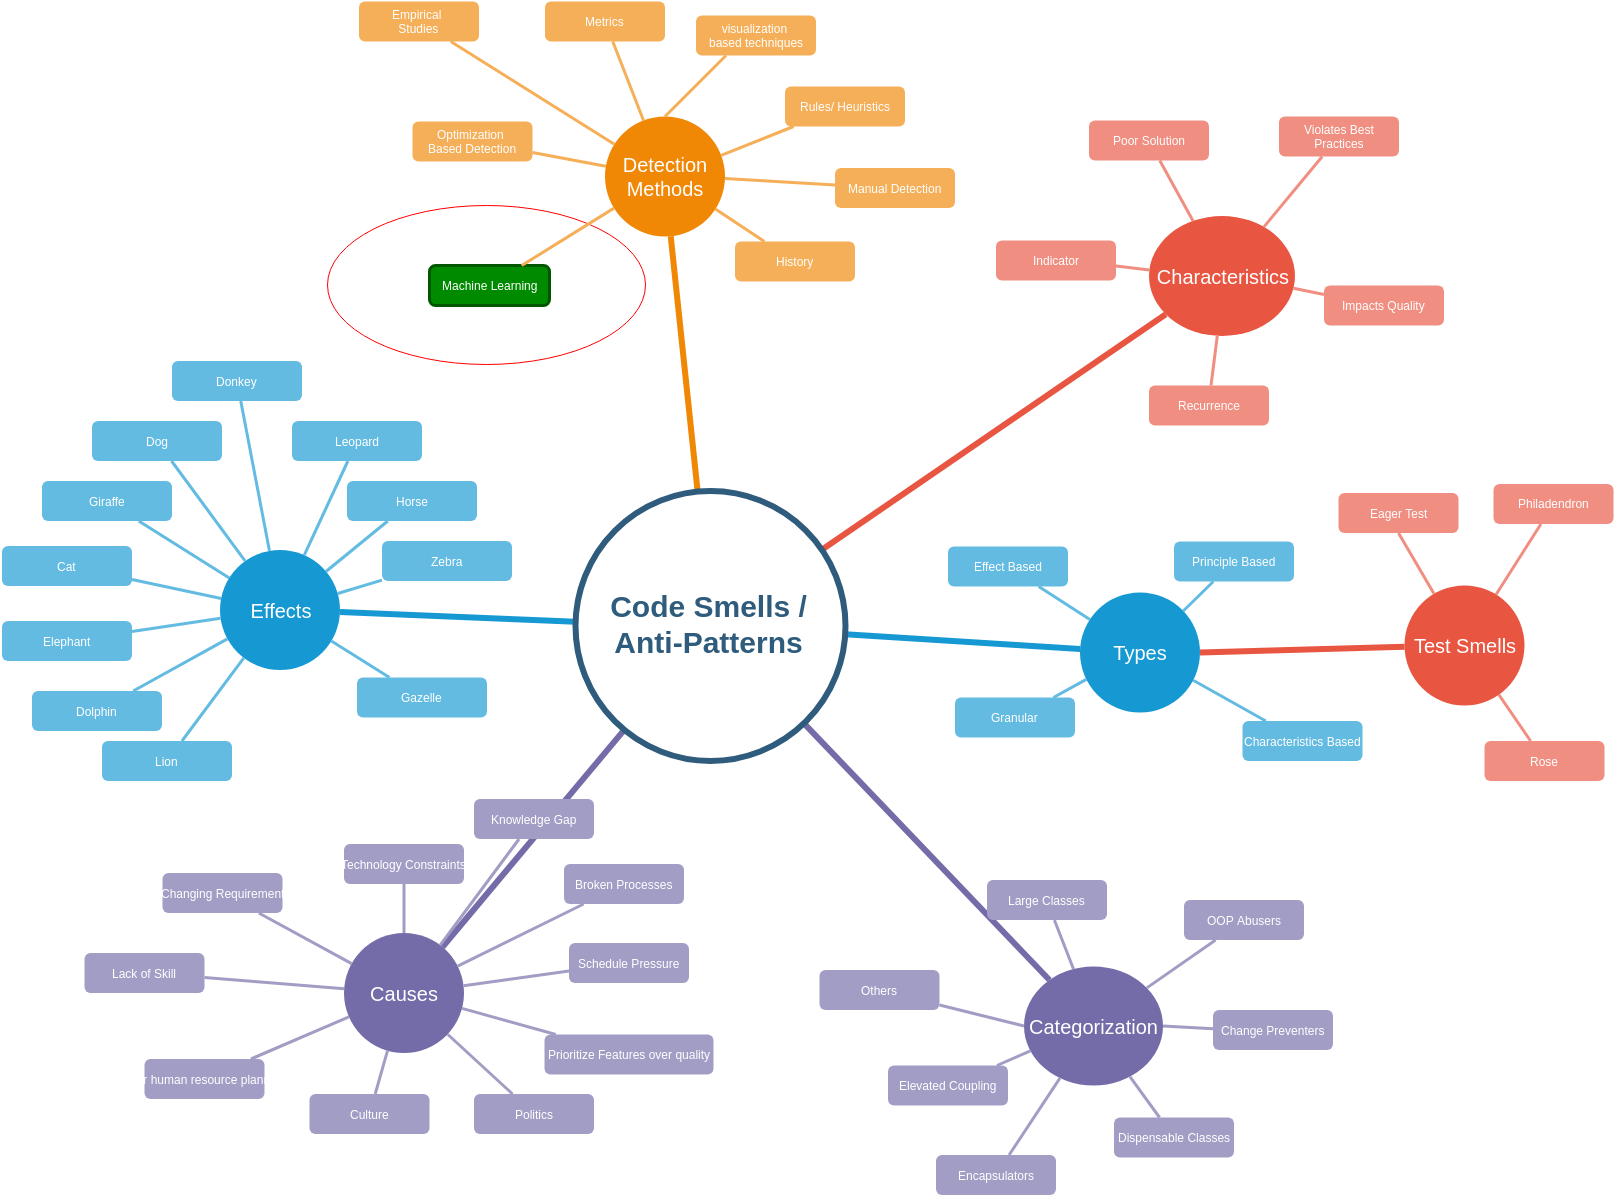
\includegraphics[width=\linewidth]{AntiPattern-TopicMap.png}}
  \caption{High level topic map on code smells and antipatterns}
  \label{fig:TM}
\end{figure*} 

\begin{figure*}[!ht]
  \centerline{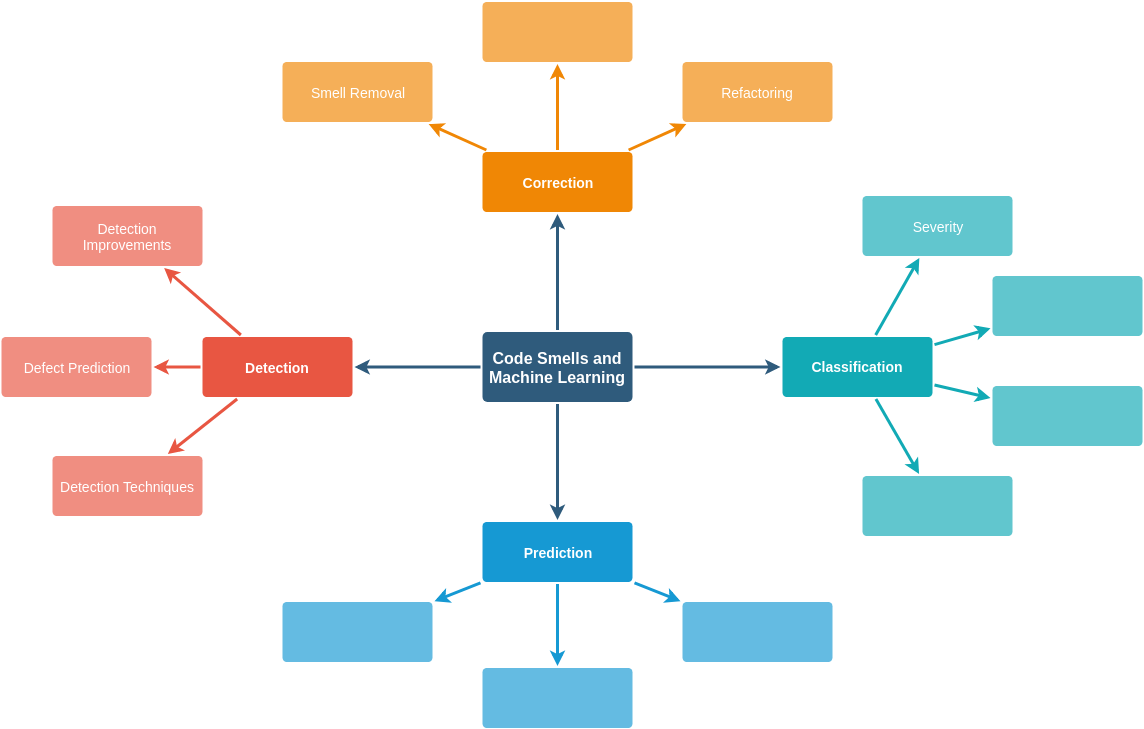
\includegraphics[width=\textwidth]{ML-codesmells.png}}
  %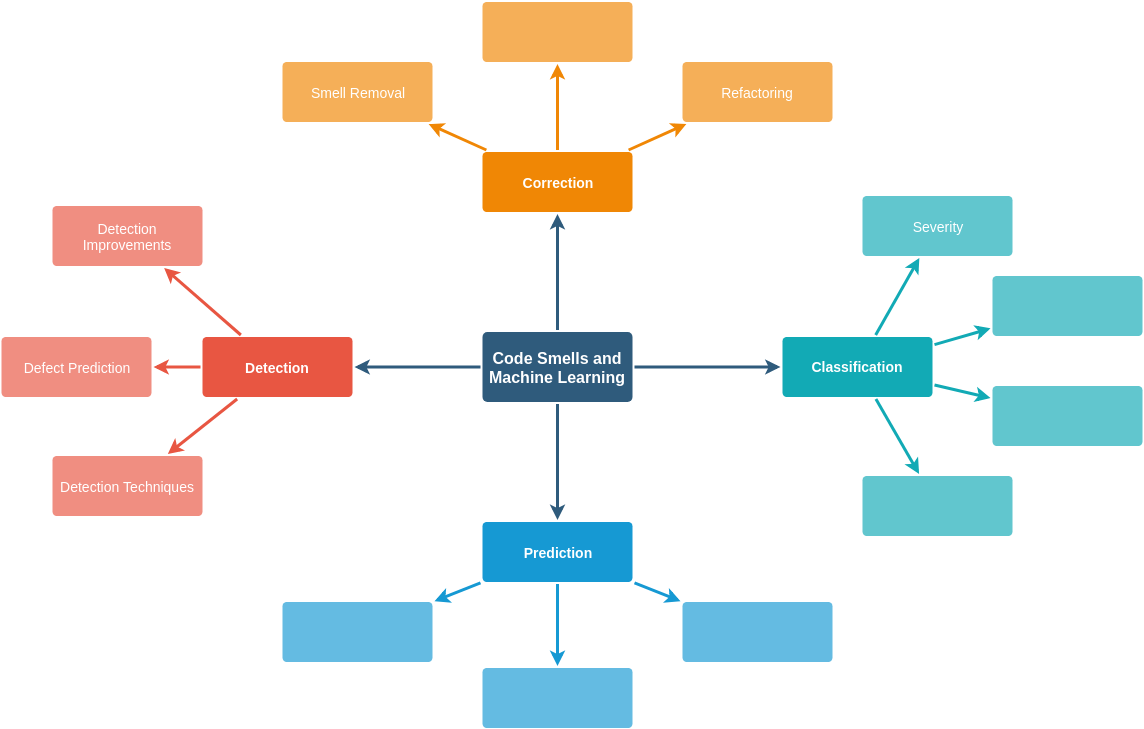
\includegraphics[width=\columnwidth]{ML-codesmells.png}
  \caption{Detail of topic map on machine learning related to code smells and antipatterns}
  \label{fig:ML}
\end{figure*} 

Include chart based on source of papers?

\section{Discussion}

\paragraph{What do the Character Need to do or Get (Goal)}
The anti-patterns need to be understood and identified.
Once that happens developers can change their best practices.
The best practices should be created in such a way that the typical misunderstandings of the developer


\paragraph{What Character Traits Make them Interesting}
What's interesting about anti-patterns is that they have a very human aspect to them. 
They overlap the way humans think with the way code is written. 
They connect common ways of human misunderstanding to software development. 
Personally, I think most developers expect code to work as they understand it to. 
They don't spend a lot of time thinking about how code will work in ways they don't expect.
It is in the nature of most engineers to see things in mathematical/binary ways and ignore the human aspects to what they are working on.
Example boeing 737 max.
Code developers expected pilots to respond with typical emergency procedure, but when the errors occurred they pilots were overwhelmed by the amount of feedback they recieved in the cockpit (need reference).
\paragraph{What Conflicts/Problems Block the Character}

The problem is people don't realize they are implementing anti-patterns at the time they are writing code.
The interesting things about it are how do we find them. 
How do we detect them, and what is the fix when we identify the problem.

\paragraph{How do they Create Risk and Danger}
Because we know that the anti-patterns cause confusion in the developer, they create risk because they create unstable code. 
This is risk for the owner of the software and the customer of the developer who uses code
\paragraph{What Does the Character Do (Struggles) to Reach Goal}
This is something I think is interesting, is how are these problems identified.
It isnt' enought to just use expert advice/knowledge. 
There must be a way to mathematically demonstrate or by experimentation that particular code patterns cause problems.

\paragraph{Who is the Main Character}
The main character is the anti-pattern. I need to find a way to clearly define the anti-pattern conceptually. 

Meaning that an anti-pattern is a known bad problem, where a code smell may lead to a problem.
An example anti-pattern is shown in listing \ref{pattern1}. Some developers will expect the output to be 25 and some will be 13 because they don't understand intuitively how the macro function works (the correct answer is 13).

On second thought, is the character the developer? 
And is what is interesting about it their human nature which leads them to confusion?
I would guess tha most developers think that a compiler is well-defined and bugs in code must be due to lack of understanding not code structure that is good at confusing human nature.

\paragraph{Why is That Goal Important (motive)}
Note: not many papers about code smells talk about why it is important.

\paragraph{What Sensory Details Will Make the Story Seem Real}
Real world examples of the problem

\section{Conclusion}

The files for this latex document are in the github repository located at \path{https://github.com/rodger79/CS6000}

\nocite{*}

%\clearpage
\bibliographystyle{IEEEtran}
\bibliography{references}


\end{document}